% The master copy of this demo dissertation is held on my filespace
% on the cl file serve (/homes/mr/teaching/demodissert/)

% Last updated by MR on 2 August 2001

\documentclass[12pt,twoside,notitlepage]{report}

\usepackage{a4}
\usepackage{verbatim}
\usepackage{pdfpages}
\input{epsf}                            % to allow postscript inclusions
% On thor and CUS read top of file:
%     /opt/TeX/lib/texmf/tex/dvips/epsf.sty
% On CL machines read:
%     /usr/lib/tex/macros/dvips/epsf.tex



\raggedbottom                           % try to avoid widows and orphans
\sloppy
\clubpenalty1000%
\widowpenalty1000%

\addtolength{\oddsidemargin}{6mm}       % adjust margins
\addtolength{\evensidemargin}{-8mm}

\renewcommand{\baselinestretch}{1.1}    % adjust line spacing to make
                                        % more readable

\begin{document}

\bibliographystyle{plain}


%%%%%%%%%%%%%%%%%%%%%%%%%%%%%%%%%%%%%%%%%%%%%%%%%%%%%%%%%%%%%%%%%%%%%%%%
% Title


\pagestyle{empty}

\hfill{\LARGE \bf Yousuf Mohamed-Ahmed}

\vspace*{60mm}
\begin{center}
\Huge
{\bf Non-contact heart rate estimation from video} \\
\vspace*{5mm}
Computer Science Tripos - Part II  \\
\vspace*{5mm}
Gonville \& Caius College\\
\vspace*{5mm}
\today  % today's date
\end{center}

\cleardoublepage

%%%%%%%%%%%%%%%%%%%%%%%%%%%%%%%%%%%%%%%%%%%%%%%%%%%%%%%%%%%%%%%%%%%%%%%%%%%%%%
% Proforma, table of contents and list of figures

\setcounter{page}{1}
\pagenumbering{roman}
\pagestyle{plain}

\chapter*{Proforma}

{\large
\begin{tabular}{ll}
Name:               & \bf Yousuf Mohamed-Ahmed \\
College:            & \bf Gonville \& Caius College                     \\
Project Title:      & \bf Non-contact heart rate estimation from video \\
Examination:        & \bf Computer Science Tripos - Part II, July 2020    \\
Word Count:         & \bf 0\footnotemark[1] \\
Project Originator: & Dr R.~Harle                    \\
Supervisor:         & Dr R.~Harle                    \\ 
\end{tabular}
}
\footnotetext[1]{This word count was computed
by the \textbf{TeXcount} script
}
\stepcounter{footnote}


\section*{Original Aims of the Project}

To write a demonstration dissertation\footnote{A normal footnote without the
complication of being in a table.} using \LaTeX\ to save
student's time when writing their own dissertations. The dissertation
should illustrate how to use the more common \LaTeX\ constructs. It
should include pictures and diagrams to show how these can be
incorporated into the dissertation.  It should contain the entire
\LaTeX\ source of the dissertation and the Makefile.  It should
explain how to construct an MSDOS disk of the dissertation in
Postscript format that can be used by the book shop for printing, and,
finally, it should have the prescribed layout and format of a diploma
dissertation.


\section*{Work Completed}

All that has been completed appears in this dissertation.

\section*{Special Difficulties}

Learning how to incorporate encapulated postscript into a \LaTeX\
document on both CUS and Thor.
 
\newpage
\section*{Declaration}

I, Yousuf Mohamed-Ahmed of Gonville \& Caius College, being a candidate for Part II of the Computer
Science Tripos, hereby declare
that this dissertation and the work described in it are my own work,
unaided except as may be specified below, and that the dissertation
does not contain material that has already been used to any substantial
extent for a comparable purpose.

\bigskip
\leftline{Signed Yousuf Mohamed-Ahmed}

\medskip
\leftline{Date \today}

\cleardoublepage

\tableofcontents

\listoffigures

\newpage
\section*{Acknowledgements}

This document owes much to an earlier version written by Simon Moore
\cite{moore95}.  His help, encouragement and advice was greatly 
appreciated.

%%%%%%%%%%%%%%%%%%%%%%%%%%%%%%%%%%%%%%%%%%%%%%%%%%%%%%%%%%%%%%%%%%%%%%%
% now for the chapters

\cleardoublepage        % just to make sure before the page numbering
                        % is changed

\setcounter{page}{1}
\pagenumbering{arabic}
\pagestyle{headings}

\chapter{Introduction}
\cleardoublepage



\chapter{Preparation}
\cleardoublepage

\chapter{Implementation}
\cleardoublepage

\chapter{Evaluation}
\cleardoublepage

\chapter{Conclusion}
\cleardoublepage

%%%%%%%%%%%%%%%%%%%%%%%%%%%%%%%%%%%%%%%%%%%%%%%%%%%%%%%%%%%%%%%%%%%%%
% the bibliography

\addcontentsline{toc}{chapter}{Bibliography}
\bibliography{refs}
\cleardoublepage

%%%%%%%%%%%%%%%%%%%%%%%%%%%%%%%%%%%%%%%%%%%%%%%%%%%%%%%%%%%%%%%%%%%%%
% the appendices
\appendix
\cleardoublepage

\chapter{Project Proposal}
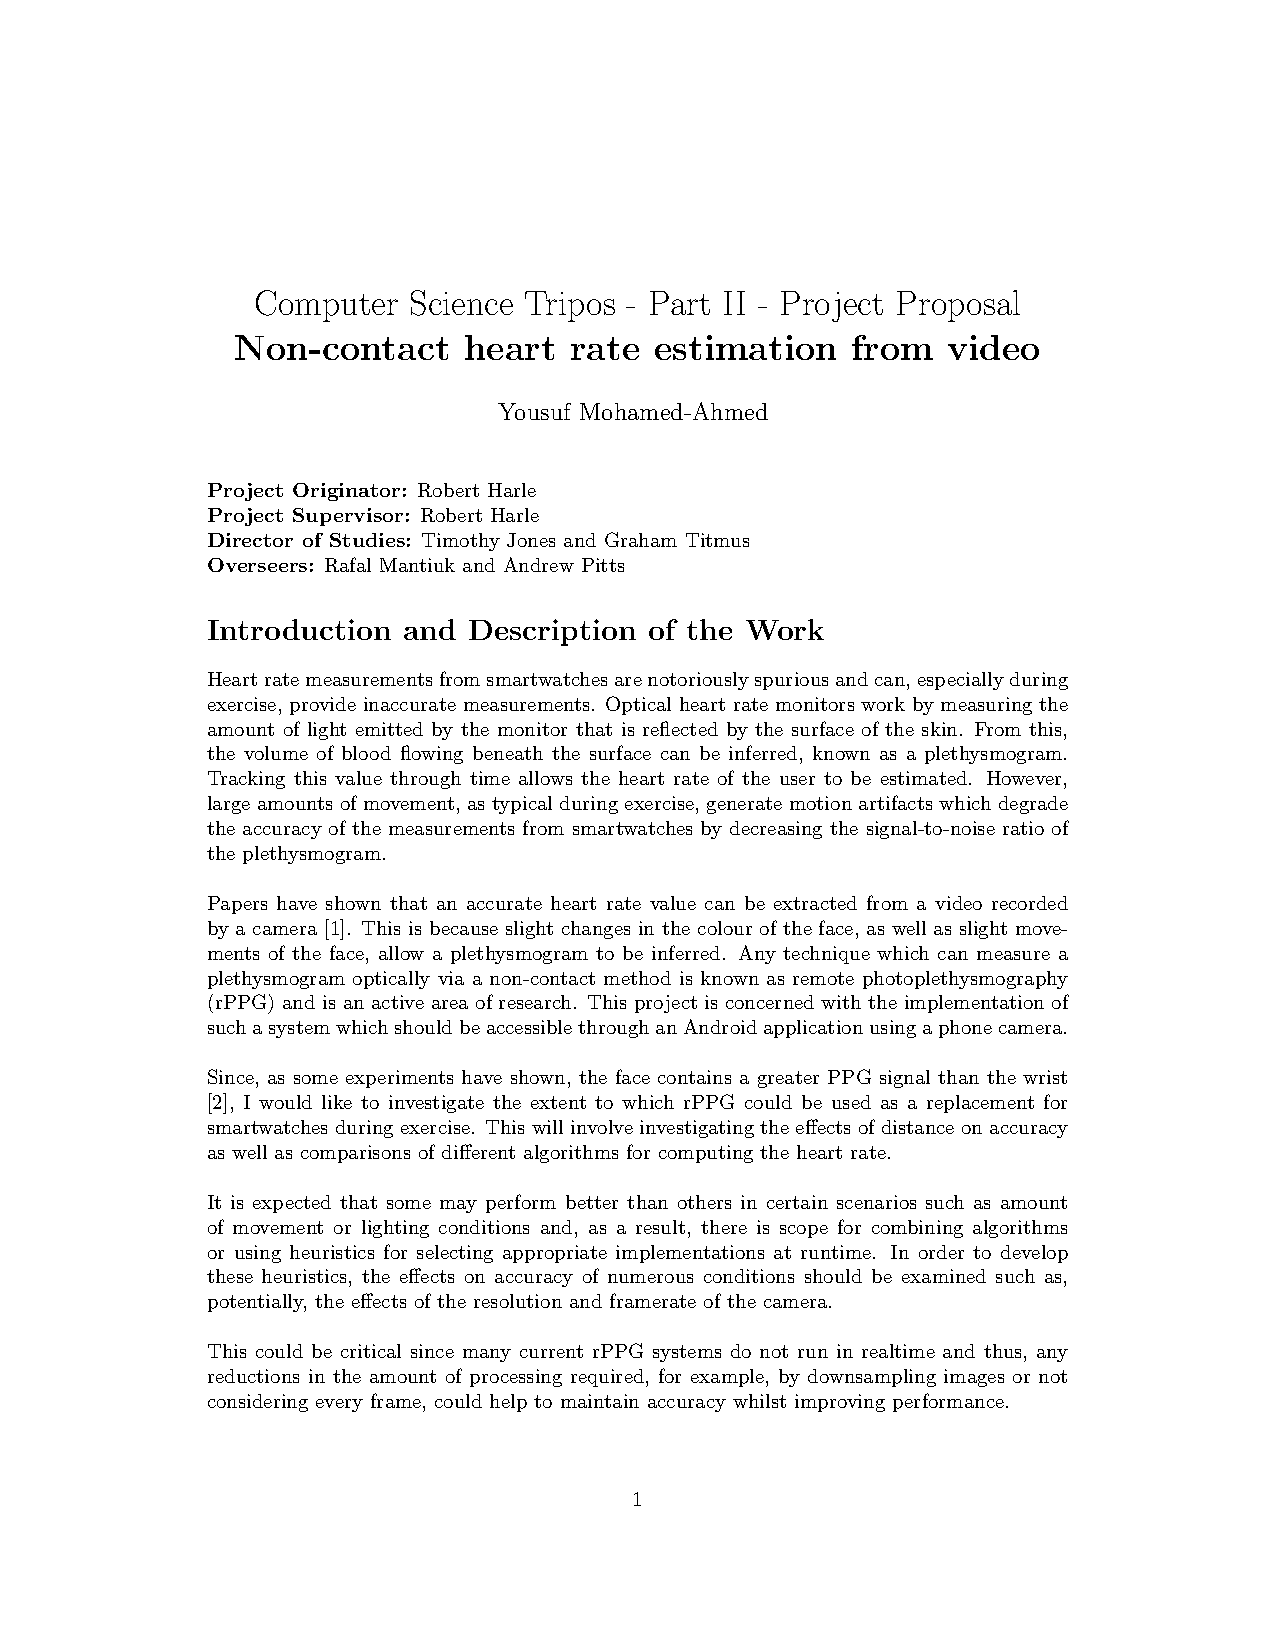
\includepdf[pages=-,pagecommand={},width=\paperwidth]{proposal/main.pdf}

\end{document}
